\chapter{Coleta e análise de dados}

Um dos processos mais críticos para o sucesso de um projeto é a obtenção de resultados e dados, dos quais se obtém conhecimento sobre o comportamento do sistema em atividade e dos usuário que o utilizam.

\section{Coleta}

Para a coleta de dados, foram usados um total de onze módulos distribuidos em locais e residências diferentes, de modo a simular maior diversidade de utilização.

\begin{enumerate}
	\item Aquário
	\item Corredor
	\item Lavanderia
	\item Sala/Cozinha
	\item Entrada
	\item Caixa d’água
	\item Victor
	\item Jarinu
	\item Daniela
	\item Hugo
	\item Gabriela
\end{enumerate}

Os módulos de 1 a 7 estão localizados na mesma residência, em Santo André. Já os módulos 9, 10 e 11 estão em casas diferentes na Grande São Paulo, e o módulo 8 está localizado na cidade de Jarinu - SP.

\begin{figure}[H]
	\centering
	\caption{Log na página do Aplicativo Backup}
	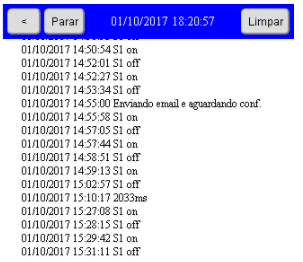
\includegraphics[width=0.5\textwidth]{logAppBackup}
	\label{fig:logAppBackup}
\end{figure}

\begin{figure}[H]
	\centering
	\caption{Módulo com cartão SD para coleta local de dados}
	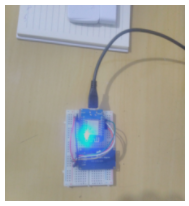
\includegraphics[width=0.3\textwidth]{SDColetaDados}
	\label{fig:SDColetaDados}
\end{figure}

Para os módulos em Santo André, foi utilizado um dispositivo com cartão SD para persistência de dados. Sua análise tem como objetivo principal acompanhar parâmetros relacionados à disponibilidade com coleta local.

\begin{figure}[H]
	\centering
	\caption{Módulos instalados em Santo André}
	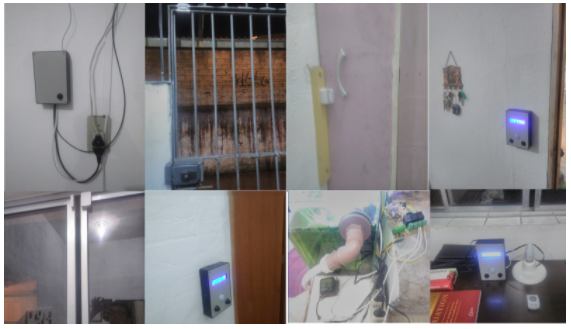
\includegraphics[width=0.8\textwidth]{ModulosStoAndre}
	\label{fig:ModulosStoAndre}
\end{figure}

O módulo de Jarinu possui uma interface com o sistema de alarmes já instalado no local e tem como objetivo obter dados de presença e abertura de portas, sendo uma prova de conceito para validar possível integração futura com parceiros estratégicos.

\begin{figure}[H]
	\centering
	\caption{Controle do Sistema de Alarme e Módulo de Interface de Jarinu}
	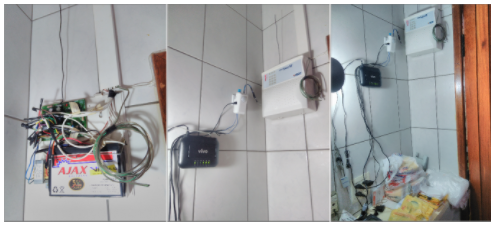
\includegraphics[width=0.8\textwidth]{ModuloSistAlarme}
	\label{fig:ModuloSistAlarme}
\end{figure}

\begin{figure}[H]
	\centering
	\caption{Módulo Básico e sensor de presença no corredor de Jarinu}
	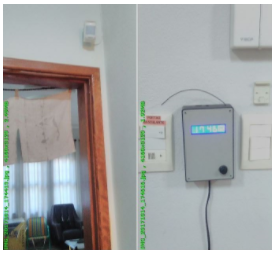
\includegraphics[width=0.5\textwidth]{BasicSensorPresJarinu}
	\label{fig:BasicSensorPresJarinu}
\end{figure}

\begin{figure}[H]
	\centering
	\caption{Sensor de abertura das portas da cozinha (à esquerda) e da sala (à direita)}
	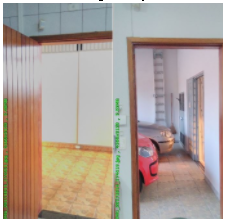
\includegraphics[width=0.5\textwidth]{SensorPortasJarinu}
	\label{fig:SensorPortasJarinu}
\end{figure}

Os demais módulos possuem coleta de dados a partir de persistência na nuvem, com as mensagens passando pelo controlador local Morpheus. Possuem como principal objetivo prover dados para o aprendizado de máquina.

\begin{figure}[H]
	\centering
	\caption{Módulo instalado para coleta de dados do nível da caixa d’água}
	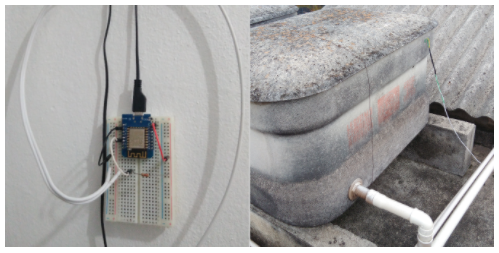
\includegraphics[width=0.8\textwidth]{ModuloCxAgua}
	\label{fig:ModuloCxAgua}
\end{figure}

Conforme destacado, os dados a seguir foram coletados localmente e possuem informações sobre disponibilidade e uso das funções pelo aplicativo backup, também com escopo local.

De modo geral, há a coleta dos seguintes dados:

\begin{figure}[H]
	\centering
	\caption{Relação dos módulos e dados coletados}
	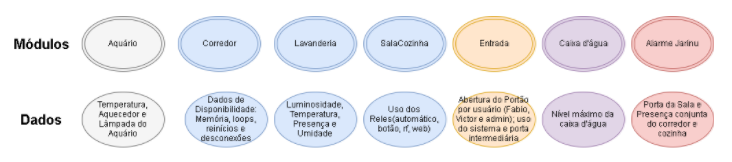
\includegraphics[width=1.0\textwidth]{DiagramaModulosDados}
	\label{fig:DiagramaModulosDados}
\end{figure}

Foram coletados dados desde o dia 10 de setembro de 2017 até o dia 13 de novembro de 2017, com processo semanal de backup. Os dados foram segregados, suas duplicatas foram removidas e os conteúdos dos diversos arquivos de log foram consolidados.

\begin{itemize}
	\item \textbf{Dados do aquário}: temperatura da água, estado do aquecedor e estado da lâmpada usada como fonte de iluminação artificial.
	\item \textbf{Dados de disponibilidade}: memória livre disponível (“\emph{free heap}”), pois em casos de pouca memória disponível, o espaço de dados invade o espaço de programa e ocorre travamento do ESP; monitoramento do contador de loops de 1 segundo que, devido à espera ou demasiado processamento, demoraram mais que 2 segundos para ocorrerem; monitoramento de desconexões, reconexões, atualizações do \emph{firmware} dos módulos e reinícios;
	\item \textbf{Luminosidade}: monitoramento a partir de dado analógico de um LDR.
	\item \textbf{Temperatura e umidade}: sensor DHT.
	\item \textbf{Presença}: sensor de presença PIR.
	\item \textbf{Uso dos relés}: pelo botão físico presente no módulo, pela página web do aplicativo backup, automaticamente por regras configuradas pelo usuário e por controle de radiofrequência (RF) --- nos módulos usados para coleta, não havia a dashboard disponível.
	\item \textbf{Abertura e estado do portão}: monitoramento do estado do portão por sensor eletromagnético com fio, conectado diretamente ao módulo, e acompanhamento das aberturas por pessoa (Fabio, Victor ou Admin, que representa alguma das outras duas pessoas da casa), uso do sistema (aberturas pelo sensor versus aberturas pelo sistema) e monitoramento de uma porta intermediária da escada, por meio de sensor de abertura sem fio (comunicação por radiofrequência).
	\item \textbf{Nível máximo da caixa d’água}: sensor de boia próximo ao nível máximo.
	\item \textbf{Porta da sala (estado) e presença (corredor e cozinha) de Jarinu}: equipamentos próprios do sistema de alarmes.

\end{itemize}

\section{Análise}

\begin{table}[H]
    \caption{Análise consolidada de disponibilidade}
    \setlength\tabcolsep{1.5pt}
    \centering
    \footnotesize
    \begin{tabular}{cccccc}
        \textbf{Item} & \textbf{Aquário} & \textbf{Corredor} & \textbf{Lavanderia} & \textbf{SalaCozinha} & \textbf{Entrada} \\
        \midrule
        memória livre [bytes] &
        30278 &
        27218 &
        26990 &
        26728 &
        26237 \\
        \# (loops) &
        1251 &
        771 &
        76 &
        925 &
        1140 \\
        \# (reinícios) &
        34 &
        18 &
        35 &
        20 &
        91 \\
        \# (desconexões do Wi-Fi) &
        15 &
        26 &
        24 &
        27 &
        77 \\
    \end{tabular}
\end{table}

O aspecto de disponibilidade foi analisado a partir da média da memória disponível --- quanto maior, melhor ---, o número de loops de 1s que ocorreram em 2s ou mais --- o que indica a existência de procedimentos que estão atrasando a correta execução de rotinas periódicas, como aquelas de “\emph{keep alive}” de comunicação ---, e o número de reinícios e desconexões da rede Wi-Fi desconsiderando aqueles causados por atualizações de \emph{firmware} dos módulos.

Como o \emph{firmware} do Corredor, Lavanderia e SalaCozinha é o mesmo (\emph{basic}), conclui-se que:

\begin{itemize}
	\item A versão aquário possui mais memória disponível, um menor número de desconexões da rede Wi-Fi e número perto da média de reinícios. Contudo, possui maior ocorrência de loops de 1s maiores que 2s, indicando algum procedimento que está consumindo tempo do loop;
	\item A versão \emph{basic} possui ocorrências de desconexões, reinícios e memória livre em valores médios;
	\item A versão \emph{entrada} possui o maior número de reinícios e desconexões da rede Wi-Fi, o que já era esperado, pois é o módulo mais longe do roteador da residência, que está em outro andar;
	\item A memória livre média das versões \emph{basic} e \emph{entrada} possuem valores próximos.
\end{itemize}

\begin{table}[H]
	\caption{Análise consolidada de uso dos relés}
	\setlength\tabcolsep{1.5pt}
	\centering
	\footnotesize
	\begin{tabular}{ccccccc}
		\textbf{Nome} &
		\textbf{Corredor} &
		\textbf{Sabrina} &
		\textbf{Varanda} &
		\textbf{Escada} &
		\textbf{Sala} &
		\textbf{Cozinha} \\
		\midrule
		\% Ligado &
		35.08\% &
		22.91\% &
		41.62\% &
		6.89\% &
		80.06\% &
		60.99\% \\
		\# Acionamentos &
		238 &
		202 &
		516 &
		382 &
		190 &
		233 \\
		\% Botão Físico &
		11.61\% &
		87.96\% &
		54.14\% &
		13.57\% &
		26.21\% &
		20.33\% \\
		\% Web &
		21.43\% &
		2.55\% &
		14.79\% &
		1.36\% &
		44.66\% &
		40.66\% \\
		\% RF &
		37.50\% &
		9.49\% &
		0.00\% &
		0.00\% &
		29.13\% &
		39.00\% \\
		\% Auto &
		29.46\% &
		0.00\% &
		31.08\% &
		85.07\% &
		0.00\% &
		0.00\% \\
	\end{tabular}
\end{table}

Quanto ao uso dos acionamentos possíveis (botão físico presente no módulo, pelo aplicativo backup - Web, por controle de radiofrequência - RF e por regra automática configurada pelo usuário - Auto), número de acionamentos e porcentagem do tempo ligado, observa-se que:

\begin{itemize}
	\item As áreas comuns têm as maiores porcentagens de tempo de lâmpadas acesas, com maiores números de acionamentos pela web, nenhum acionamento por regra automática, dobro de acionamentos por RF em relação ao botão físico para a lâmpada da cozinha e números de acionamentos por RF e botão físico em valores próximos para a Sala;
	\item A escada tem o melhor uso do acionamento automático, indicando que a regra de acender a lâmpada da escada quando a porta de entrada abrir em horário noturno é bem empregada;
	\item Para a lâmpada da varanda, ainda que com um bom uso automático, cerca de metade dos acionamentos ainda ocorre por meio do botão físico;
	\item Quarto da Sabrina possui nenhum uso de acionamento automático e poucos acionamentos pela web (celular) e controle RF, indicando que o sistema não agrega muito valor;
	\item Lâmpada do corredor possui uma distribuição aproximadamente igualitária entre os acionamentos, contrariando o comportamento esperado de que as regras automáticas de acendimento de luz quando da presença detectada seriam suficientes para o controle dessa lâmpada;
	\item O uso de acionamentos pelo aplicativo (web) somente são consideráveis nas áreas comuns, provavelmente referindo-se a quando os usuários desligam as luzes da casa toda antes de dormir. Pode-se considerar que, apesar de ser um meio adequado de apresentar o funcionamento do sistema, no uso cotidiano os usuários preferem usar controles RF, acionamento manual por botão físico ou deixar uma regra para atuação automática.
\end{itemize}

\begin{figure}[H]
	\centering
	\caption{Curva diária Santo André -- terça-feira}
	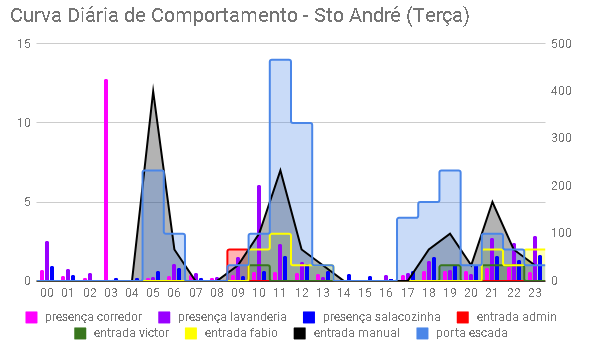
\includegraphics[width=0.8\textwidth]{diaStoAndreTerca}
	\label{fig:diaStoAndreTerca}
\end{figure}

Tomando o dia de terça-feira como exemplo dos gráficos consolidados de Santo André, observa-se que:

\begin{itemize}
	\item Há um pico de presença no corredor às 3h. Seria o horário em que os gatos da residência estão mais ativos;
	\item A curva de presença indica maiores movimentos entre 9h e 13h e entre 17h e 1h, horários em que as pessoas entram ou saem da residência;
	\item A curva de presença indica maiores movimentos entre 9h e 13h e entre 17h e 1h, horários em que as pessoas entram ou saem da residência;
	\item Considerando que a segmentação de usuários da entrada está em Fabio, Victor e Admin (Nair e Sabrina):
	\begin{itemize}
		\item Das 4h às 7h, Nair/Sabrina sai da casa;
		\item Das 9h às 13h, Fabio sai de casa, algumas vezes usando seu usuário, outras vezes manualmente;
		\item Às 10h, Victor sai de casa;
		\item Das 17h às 19h, Sabrina/Nair voltam para casa;
		\item Entre 19h e 22h, Victor volta para casa;
		\item Entre 21h e 23h, Fabio volta para casa;
	\end{itemize}
	\item Os picos de porta escada indicam os horários de maior entrada e saída da residência.
\end{itemize}

\begin{figure}[H]
	\centering
	\caption{Temperatura e aquecedor -- Módulo do Aquário}
	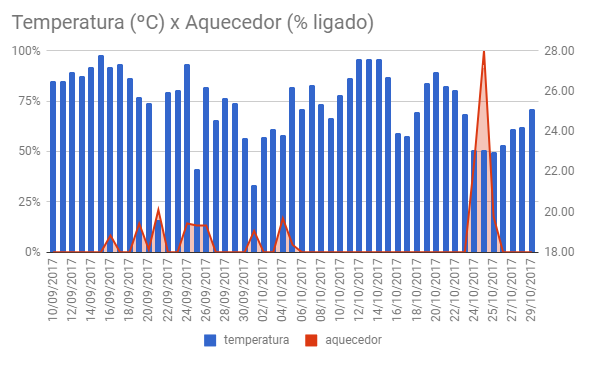
\includegraphics[width=1.0\textwidth]{TempAquecedorAqua}
	\label{fig:TempAquecedorAqua}
\end{figure}

Considerando a curva diária e histórico do período dos sensores e atuador do aquário, observa-se que:

\begin{itemize}
	\item Às 3h da manhã, a lâmpada está acesa e aquecedor, ligado. Isso pode ter ocorrido em um dia em particular (25/11/2017, dia atípico, como observado no gráfico do período);
	\item Das 9h às 23h, há uma regra para que a lâmpada do aquário fique acesa;
	\item A temperatura é menor às 10h e das 14h às 18h. O comportamento do aquecedor é no sentido de ligar nesses períodos.

\end{itemize}

\begin{figure}[H]
	\centering
	\caption{Consolidado Diário -- Módulo do Aquário}
	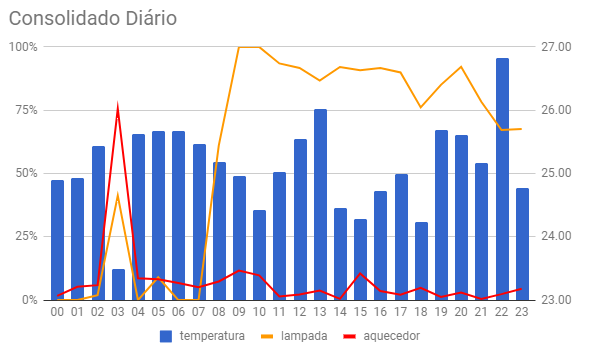
\includegraphics[width=1.0\textwidth]{AquaDia}
	\label{fig:AquaDia}
\end{figure}

\begin{figure}[H]
	\centering
	\caption{Memória e loops -- Módulo do Corredor}
	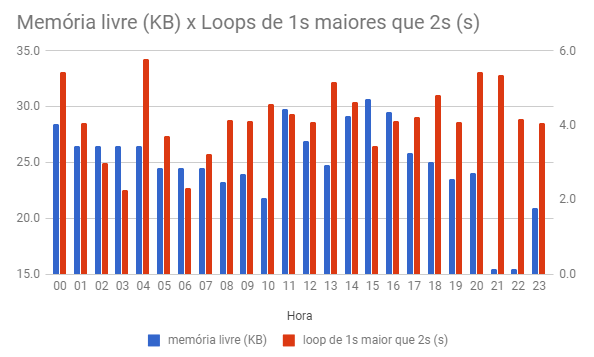
\includegraphics[width=1.0\textwidth]{MemLivreCorredor}
	\label{fig:MemLivreCorredor}
\end{figure}

Observando sua curva diária de memória livre e loops de 1s que foram executados em mais de 2s, observou-se que:

\begin{itemize}
	\item Os períodos de maior disponibilidade são das 11h às 16h, pois há maior memória livre, que é o parâmetro mais crítico para possíveis reinícios e travamentos;
	\item Os períodos de menor disponibilidade são das 21h às 22h, nos quais houve picos de loops demorados e pouquíssima memória livre.
\end{itemize}

\begin{figure}[H]
	\centering
	\caption{Consolidado no período -- Módulo do Corredor}
	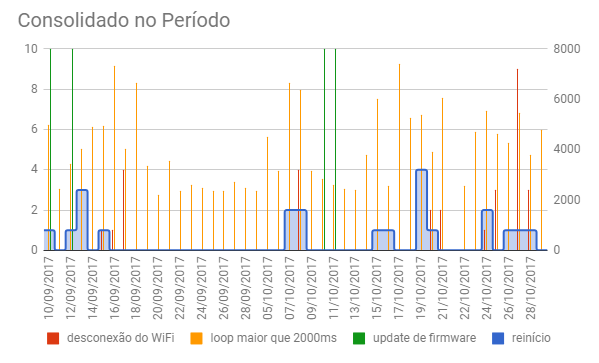
\includegraphics[width=1.0\textwidth]{periodoCorredor}
	\label{fig:periodoCorredor}
\end{figure}

São observados em verde, no gráfico acima, as atualizações de \emph{firmware} --- o que possibilita acompanhar a melhoria de disponibilidade após a implantação de novas versões ---, a quantidade de reinícios e ocorrências de desconexão do Wi-Fi. Entre 24/10 e 28/10, ocorreu grande número de desconexões do Wi-Fi, indicando indisponibilidade da rede nesses dias, que causaram certa quantidade de reinícios no mesmo período.

\begin{figure}[H]
	\centering
	\caption{Consolidado diário dos sensores -- Módulo do Corredor}
	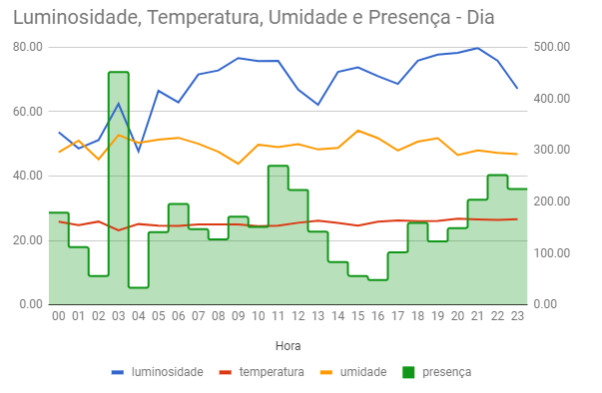
\includegraphics[width=1.0\textwidth]{sensoresdiaCorredor}
	\label{fig:sensoresdiaCorredor}
\end{figure}

No gráfico acima, observa-se inatividade às 4h da manhã e entre as 14h e 16h. A temperatura possui pouca variação, assim como a umidade. Já a curva de luminosidade acompanha a de presença. Apenas das 14h às 16h, considere que há luz natural, por isso não é um valor próximo àquele apresentado de madrugada, entre 0h e 4h.

\begin{figure}[H]
	\centering
	\caption{Uso dos acionamentos no período para a lâmpada -- Módulo do Corredor}
	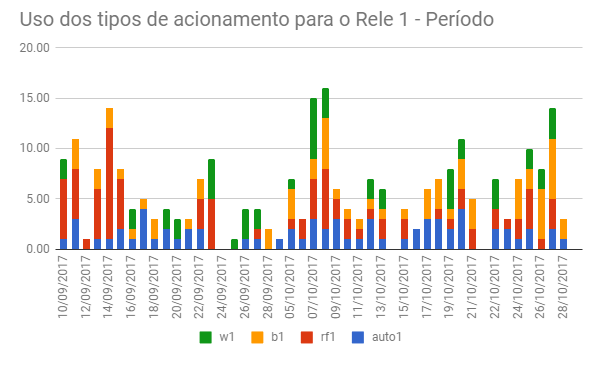
\includegraphics[width=1.0\textwidth]{UsoRele1periodoCorredor}
	\label{fig:UsoRele1periodoCorredor}
\end{figure}

No primeiro gráfico, observa-se a evolução do uso dos acionamentos para o relé 1 (lâmpada do corredor) no período. Observam-se dias com maiores e menores quantidades de acionamentos e a participação das regras automáticas em relação aos outros tipos de acionamento. No segundo, verifica-se que, durante o dia, os acionamentos automáticos ocorrem entre 17h e 22h. Possivelmente, podem-se aplicar regras no período das 23h às 2h.

\begin{figure}[H]
	\centering
	\caption{Uso dos acionamentos por dia para a lâmpada -- Módulo do Corredor}
	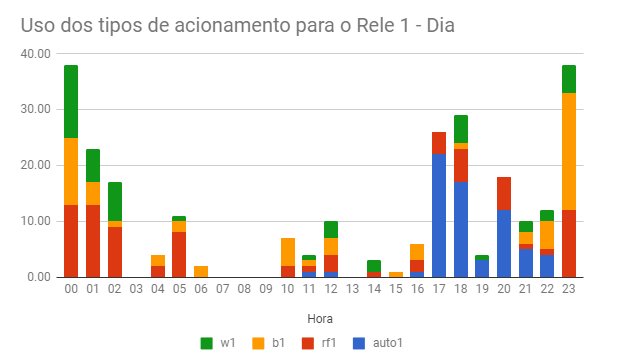
\includegraphics[width=0.8\textwidth]{UsoRele1DiaCorredor}
	\label{fig:UsoRele1DiaCorredor}
\end{figure}

\begin{figure}[H]
	\centering
	\caption{Curva diária -- Módulo de Acesso}
	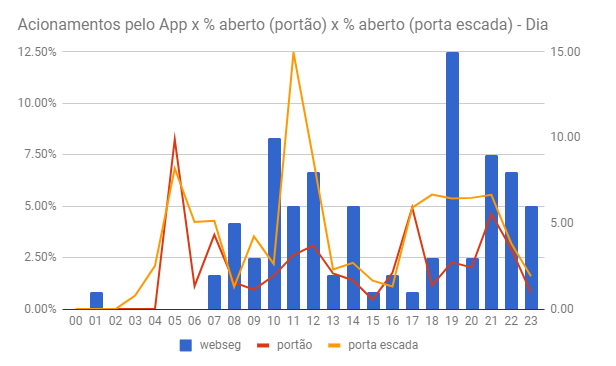
\includegraphics[width=1.0\textwidth]{EntradaConsolidadoDia}
	\label{fig:EntradaConsolidadoDia}
\end{figure}

Com a curva diária de comportamento para o módulo de entrada, observa-se que:

\begin{itemize}
	\item Os horários com maior número de acionamentos pelo celular são 10h, 12h, 19h, 21h, 22h e 23h;
	\item Usuários que entram ou saem de casa às 17h não usam o celular para abrir o portão, tampouco aqueles que entram ou saem às 5h.
\end{itemize}

\begin{figure}[H]
	\centering
	\caption{Nível da caixa d'água -- consolidado diário}
	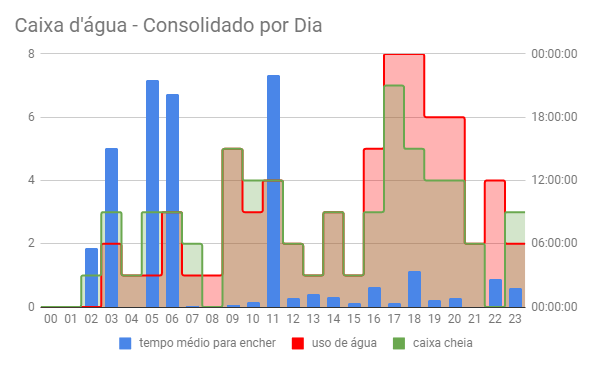
\includegraphics[width=1.0\textwidth]{CxAguaDia}
	\label{fig:CxAguaDia}
\end{figure}

Na curva diária do módulo da caixa d’água, nota-se que:

\begin{itemize}
	\item Há maior uso de água, provavelmente para banho, nos períodos das 9h às 12h e entre 16h e 23h;
	\item Os horários em que provavelmente há menor disponibilidade de água da rua para preencher a caixa e fazer o nível voltar a ser alto são das 5h às 6h da manhã e às 11h da manhã.

\end{itemize}

Observando o gráfico a seguir, observam-se os dias em que houve falta de água  --- picos de demora para preencher a caixa de água após algum uso perceptível pelo sensor do tipo boia.

\begin{figure}[H]
	\centering
	\caption{Tempo para encher a caixa d'água -- período}
	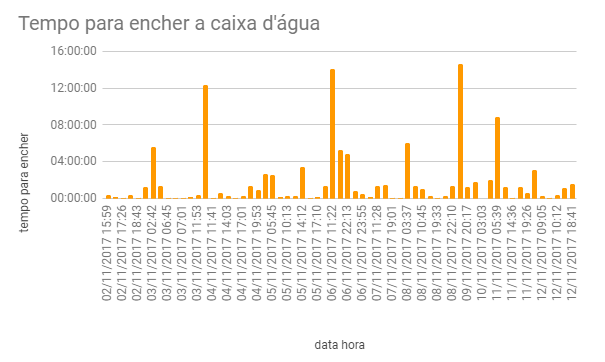
\includegraphics[width=1.0\textwidth]{tempoPeriodocxAgua}
	\label{fig:tempoPeriodocxAgua}
\end{figure}

\begin{figure}[H]
	\centering
	\caption{Atividade da porta -- Sala de Jarinu}
	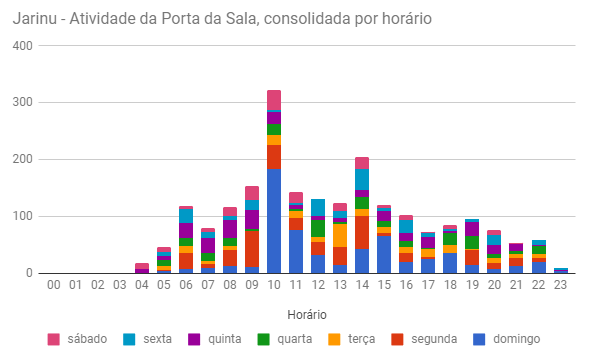
\includegraphics[width=1.0\textwidth]{AtivPortaSalaJarinu}
	\label{fig:AtivPortaSalaJarinu}
\end{figure}

Em Jarinu, um idoso com boa saúde física mora sozinho em sua residência. Ao analisar as curvas diárias de atividade da porta da sala e presença, notou-se:

\begin{itemize}
	\item Atividade de presença ente 4h e 5h da manhã, entre 10h e 12h e entre 16h e 20h.
	\item Atividade de presença maior em domingos, segundas e terças;
	\item Grande atividade da porta da sala às 10h e 14h. O pico das 10h ocorre principalmente aos domingos.
\end{itemize}

\begin{figure}[H]
	\centering
	\caption{Atividade da presença -- Sala de Jarinu}
	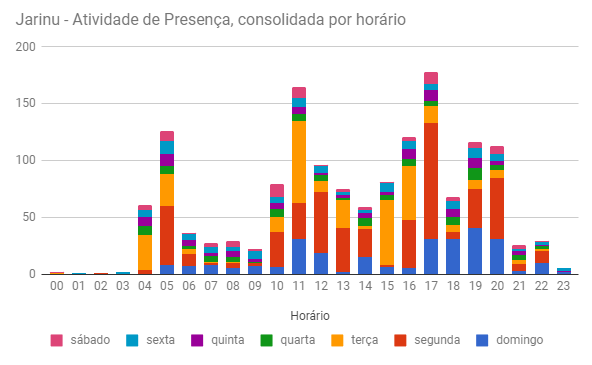
\includegraphics[width=1.0\textwidth]{AtivPresencaJarinu}
	\label{fig:AtivPresencaJarinu}
\end{figure}

\begin{figure}[H]
	\centering
	\caption{Consolidado no período -- Jarinu}
	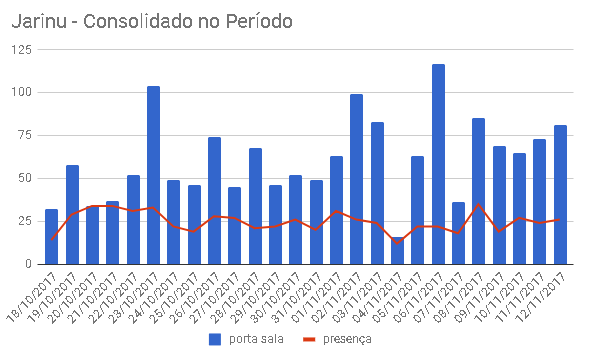
\includegraphics[width=1.0\textwidth]{JarinuPeriodo}
	\label{fig:JarinuPeriodo}
\end{figure}

Ao analisar por período, pode-se verificar o aumento ou diminuição de atividade, o que pode ser um indicativo de bem-estar. Por exemplo, no gráfico acima verifica-se que o dia 04/11 foi um dia atípico, com menores presença e atividade da porta da sala. Em geral, não houve tendência de crescimento ou diminuição do nível de atividade geral no período observado.
